%%%%%%%%%%%%%%%%%%%%%%%%%%%%%%%%%%%
%This is the LaTeX ARTICLE template for RSC journals
%Copyright The Royal Society of Chemistry 2016
%%%%%%%%%%%%%%%%%%%%%%%%%%%%%%%%%%%

\documentclass[twoside,twocolumn,9pt]{article}
\usepackage{extsizes}
\usepackage[super,sort&compress,comma]{natbib}
\usepackage[version=4]{mhchem}
\usepackage[left=1.5cm, right=1.5cm, top=1.785cm, bottom=2.0cm]{geometry}
\usepackage{balance}
\usepackage{times,mathptmx}
\usepackage{sectsty}
\usepackage{graphicx}
\usepackage{lastpage}
\usepackage[format=plain,justification=justified,singlelinecheck=false,font={stretch=1.125,small,sf},labelfont=bf,labelsep=space]{caption}
\usepackage{float}
\usepackage{fancyhdr}
\usepackage{fnpos}
\usepackage[english]{babel}
\addto{\captionsenglish}{%
  \renewcommand{\refname}{Notes and references}
}
\usepackage{array}
\usepackage{droidsans}
\usepackage{charter}
\usepackage[T1]{fontenc}
\usepackage[usenames,dvipsnames]{xcolor}
\usepackage{setspace}
\usepackage[compact]{titlesec}
\usepackage{hyperref}
% Shawn's packages
\usepackage{upgreek}
\usepackage{chemformula}
\usepackage{wasysym}
%%%Please don't disable any packages in the preamble, as this may cause the template to display incorrectly.%%%

\usepackage{epstopdf}%This line makes .eps figures into .pdf - please comment out if not required.

% Personal pacakages that I use:
\usepackage{enumitem}

\definecolor{cream}{RGB}{222,217,201}

\graphicspath{{figures/}{figures/Alternates/}}
\begin{document}

\pagestyle{fancy}
\thispagestyle{plain}
\fancypagestyle{plain}{

%%%HEADER%%%
\fancyhead[C]{
\includegraphics[width=18.5cm]{head_foot/header_bar}}
\fancyhead[L]{\hspace{0cm}\vspace{1.5cm}
\includegraphics[height=30pt]{head_foot/journal_name}}
\fancyhead[R]{\hspace{0cm}\vspace{1.7cm}
\includegraphics[height=55pt]{head_foot/RSC_LOGO_CMYK}}
\renewcommand{\headrulewidth}{0pt}
}
%%%END OF HEADER%%%

%%%PAGE SETUP - Please do not change any commands within this section%%%
\makeFNbottom
\makeatletter
\renewcommand\LARGE{\@setfontsize\LARGE{15pt}{17}}
\renewcommand\Large{\@setfontsize\Large{12pt}{14}}
\renewcommand\large{\@setfontsize\large{10pt}{12}}
\renewcommand\footnotesize{\@setfontsize\footnotesize{7pt}{10}}
\makeatother

\renewcommand{\thefootnote}{\fnsymbol{footnote}}
\renewcommand\footnoterule{\vspace*{1pt}%
\color{cream}\hrule width 3.5in height 0.4pt \color{black}\vspace*{5pt}}
\setcounter{secnumdepth}{5}

\makeatletter
\renewcommand\@biblabel[1]{#1}
\renewcommand\@makefntext[1]%
{\noindent\makebox[0pt][r]{\@thefnmark\,}#1}
\makeatother
\renewcommand{\figurename}{\small{Fig.}~}
\sectionfont{\sffamily\Large}
\subsectionfont{\normalsize}
\subsubsectionfont{\bf}
\setstretch{1.125} %In particular, please do not alter this line.
\setlength{\skip\footins}{0.8cm}
\setlength{\footnotesep}{0.25cm}
\setlength{\jot}{10pt}
\titlespacing*{\section}{0pt}{4pt}{4pt}
\titlespacing*{\subsection}{0pt}{15pt}{1pt}
%%%END OF PAGE SETUP%%%

%%%FOOTER%%%
\fancyfoot{}
\fancyfoot[LO,RE]{\vspace{-7.1pt}
\includegraphics[height=9pt]{head_foot/LF}}
\fancyfoot[CO]{\vspace{-7.1pt}\hspace{13.2cm}
\includegraphics{head_foot/RF}}
\fancyfoot[CE]{\vspace{-7.2pt}\hspace{-14.2cm}
\includegraphics{head_foot/RF}}
\fancyfoot[RO]{\footnotesize{\sffamily{1--\pageref{LastPage} ~\textbar  \hspace{2pt}\thepage}}}
\fancyfoot[LE]{\footnotesize{\sffamily{\thepage~\textbar\hspace{3.45cm} 1--\pageref{LastPage}}}}
\fancyhead{}
\renewcommand{\headrulewidth}{0pt}
\renewcommand{\footrulewidth}{0pt}
\setlength{\arrayrulewidth}{1pt}
\setlength{\columnsep}{6.5mm}
\setlength\bibsep{1pt}
%%%END OF FOOTER%%%

%%%FIGURE SETUP - please do not change any commands within this section%%%
\makeatletter
\newlength{\figrulesep}
\setlength{\figrulesep}{0.5\textfloatsep}

\newcommand{\topfigrule}{\vspace*{-1pt}%
\noindent{\color{cream}\rule[-\figrulesep]{\columnwidth}{1.5pt}} }

\newcommand{\botfigrule}{\vspace*{-2pt}%
\noindent{\color{cream}\rule[\figrulesep]{\columnwidth}{1.5pt}} }

\newcommand{\dblfigrule}{\vspace*{-1pt}%
\noindent{\color{cream}\rule[-\figrulesep]{\textwidth}{1.5pt}} }

\makeatother
%%%END OF FIGURE SETUP%%%

%%%TITLE, AUTHORS AND ABSTRACT%%%
\twocolumn[
  \begin{@twocolumnfalse}
\vspace{3cm}
\sffamily
\begin{tabular}{m{4.5cm} p{13.5cm} }


\includegraphics{head_foot/DOI} & \noindent\LARGE{\textbf{Kinetic Modeling of the \textit{Arabidopsis thaliana} Cryptochrome 1
Photocycle in Alternating Light and Magnetic Field Conditions$^\dag$}} \\
\vspace{0.3cm} & \vspace{0.3cm} \\

& \noindent\large{Shawn Strausser\textit{$^{a}$} and Thorsten Ritz$^{\ast}$\textit{$^{a}$}} \\


\includegraphics{head_foot/dates} & \noindent\normalsize{Experimental tests of \textit{Arabidopsis thaliana} cryptochrome have
recently studied the interplay between magnetic and light stimuli when both are allowed to flicker. Here we present kinetic
calculations of the size of magnetic field effects (MFE's) based on the established photocycle of cryptochrome and a simple 
phosphorylation model. In the calculations, as in the experiments, the light source undergoes cycles between on and off, while 
three magnetic scenarios are distinguished: (1) magnetic field only on during light, (2) magnetic field only on during the dark, 
(3) magnetic field on during both the light and dark periods. The calculations support the interpretation that the magnetically 
sensitive step occurs in the dark and provide a good match with experimental results. We also explore the interdependence between 
system and experimentally changeable parameters and demonstrate that relatively modest changes in parameters can lead to 
qualitatively different results especially in scenario (1)}

\end{tabular}

 \end{@twocolumnfalse} \vspace{0.6cm}

  ]
%%%END OF TITLE, AUTHORS AND ABSTRACT%%%

%%%FONT SETUP - please do not change any commands within this section
\renewcommand*\rmdefault{bch}\normalfont\upshape
\rmfamily
\section*{}
\vspace{-1cm}

%%%FOOTNOTES%%%

\footnotetext{\textit{$^{a}$~Department of Physics and Astronomy, University of California, Irvine, Ca 92697}}
\footnotetext{\textit{$^{*}$ To whom correspondence should be addressed: tritz@uci.edu}}

%Please use \dag to cite the ESI in the main text of the article.
%If you article does not have ESI please remove the the \dag symbol from the title and the footnotetext below.
\footnotetext{\dag~Electronic Supplementary Information (ESI) available: [details of any supplementary information available should
be included here]. See DOI: 00.0000/00000000.}

%%%END OF FOOTNOTES%%%

%%%MAIN TEXT%%%%
\section{Introduction}
The biophysical basis for natural magneto-sensation remains a mystery despite more than four decades of research since the seminal
discovery of a magnetic compass in birds. \cite{Wiltschko72} Behavioral studies indicate that magnetic sensing is widespread among
animals and magnetic compasses have been found not only in migratory and non-migratory birds (chicken, zebrafinch, pigeons), but
also in sea turtles,\cite{Lohmann1991} fish,\cite{Quinn1980, Walker2006} insects, salamanders, and even mammals, \cite{Begall2013}
to name a few examples.

Theoretically, the use of specialized, photo-activated, chemical reactions (radical-pair mechanism), has emerged as one of the two
frontrunners among the biologically credible mechanisms for detecting earth-strength magnetic fields (the other one being the use of
small iron-containing particles \cite{Kirschvink1981}). In the radical pair mechanism \cite{Schulten1978} a pair of radicals is
created, e.g., by an electron transfer reaction, in a coherent two-electron-spin state which may be either singlet (S) or triplet
(T). The spin states change under the influence of local magnetic fields (e.g.\ hyperfine interactions of the electron spins with
magnetic nuclei) and Zeeman interactions of electron spins with an external magnetic field. The relative yield of chemically
distinct products formed from either the S or T states are thus dependent on the external magnetic field. The theory of the radical
pair mechanism is well developed and has been successfully used over the last 40 years for the quantitative interpretation of a
variety of experimental data. Within the context of a photoreceptor molecule, the effect of the magnetic field would be manifested
by either speeding up or slowing down a light-activated reaction step that involves a radical-pair intermediate. In other words, the
magnetic field effect would be equivalent to a change in light intensity and one therefore expects an interplay of light and
magnetic field effects on a putative photo-magnetoreceptor.

Indeed, it was found in a series of studies that the magnetic compass of birds is light-dependent with a complex non-monotonic
dependence on the ambient light conditions. \cite{Johnsen2007, Wiltschko2016, Wiltschko2008} The radical-pair mechanism received
greatly increased interest following the proposal that the magnetosensitive radical reactions may occur in cryptochrome (Cry)
photoreceptors located in the eyes of birds \cite{Ritz2000} with an overview of the current state of research recently published.
\cite{Hore2016}

Cryptochromes are flavoprotein receptors found throughout the biological kingdom with important signaling functions in plants and
animals. \cite{Chaves2011} Their molecular structure and primary photoreactions are highly conserved, suggesting a common mechanism
of biological activation. For instance, in the case of plant Crys, the receptor adopts a closed conformational state in the dark to
which flavin is bound in the oxidized redox state ($\text{FAD}_{\text{ox}}$)(Fig.~\ref{fig:photocycle}). \cite{Ahmad2016} Upon
illumination, flavin undergoes a photochemical reaction to produce reduced flavin intermediates $\ce{FADH^{.}}$ and $\ce{FADH^{-}}$
(Panel A). This process in turn triggers a conformational change in the Cry protein surface (Panel B), enabling access for
transcription factors, kinases, and other cellular signaling intermediates to initiate plant growth and other responses to light. An
essentially similar signaling mechanism occurs for Drosophila Cry (DmCry), where flavin reduction ($\text{FAD}_{\text{ox}}$ to
$\ce{FADH^{.-}}$) has been shown as necessary and sufficient for structural change. This enables the binding of cellular
intermediates such as clock proteins that mediate downstream biological signaling responses. \cite{Vaidya2013}

In the original suggestion, \cite{Ritz2000} the magnetically sensitive reaction was suggested to occur during the FAD to
$\ce{FADH^{.}}$ transition in Cry photoactivation, which involves formation of Flavin-Trp radical pairs by electron transfers. Many
studies have focused on the physio-chemical properties of these radical pairs \cite{Atkins2019, Solovyov2007, Biskup2009,
	Sheppard2017} and Trps in the electron transfer chains were used as targets for mutation studies of animal magnetic sensitivity.
\cite{Gegear2010, Fedele2014} A second possible magnetically sensitive radical pair reaction could occur during the dark reoxidation
step. Several possible radical pairs have been suggested for reoxidation from the fully reduced form $\ce{FADH^{-}}$ state
\cite{Ritz2009, FADH-Z RP}. Here we do not attempt to speculate about the concrete chemical nature of the possible radical pair.
Rather, we assume that the effect of the as of yet unknown radical pair will be to change the speed of the reoxidation step from
$\ce{FADH^{.}}$ to $\text{FAD}_{\text{ox}}$ which generates the resting state. This approach is motivated by several recent
experiments using varying light conditions in behavioral or physiological experiments to identify the reaction step modified by an
applied magnetic field. In the first of these studies, birds were kept under full spectrum light before being transported to a test
arena where their ability to orient magnetically was tested in either 424 nm blue, 502 nm turquoise, or 565 nm green light.
\cite{Wiltschko2014} When birds were tested immediately after being kept in full spectrum light, they were able to orient in all
three light conditions. However, if birds were kept for 1h in darkness prior to testing in the three light conditions, they orient
in the correct migratory direction only in the blue and turquoise conditions, but not in the green condition. This can be
rationalized in the context of Cry if one assumes that the magnetically sensitive reaction step occurs during the dark re-oxidation.
The requirement is that a pool of semi-reduced or fully reduced flavin exists during the experiment. Under blue and turquoise light,
Cry can be photoreduced, but not under green light. Following light exposure, it could be seen that activated Cry1a can be found in
birds after 30 mins, but not after 1h. \cite{Niessner2013, Niessner2014} Assuming that birds make an orientation decision soon after
they are placed in the test arena, birds should therefore be able to orient in green light when tested immediately after light
exposure, but not after 1h of darkness, as was observed in the experiments. \cite{Wiltschko2014} In follow-up studies, a slightly
different protocol has been used using flicker light conditions. The basic idea is to alternate light and dark periods and to
correlate the magnetic stimulus with only one of the periods, so as to probe which part of the photocycle is involved in mediating
magnetic field effects. Typically, flicker light conditions begin with a light period $t_{\textsc{l}}$ meant to activate Cry by
driving $\text{FAD}_{\text{ox}}$ - $\ce{FADH^{.}}$ transitions in the absence of a magnetic stimulus, which is followed by a dark
period $t_{\textsc{d}}$ with the magnetic stimulus applied. In some experimental protocols, a small pause period with darkness and
no magnetic stimulus is inserted between these two periods. In European robins, it was found that under flicker light conditions
with $t_{\textsc{l}}$ = 300 ms (light on, no magnetic field) and $t_{\textsc{d}}$ = 700 ms (light off, magnetic field on), birds
were able to orient both in 502 nm turquoise and 565 nm green light.
In addition to studying the magnetic compass of birds with its unknown magnetic receptor, two recent studies have employed flicker
lights to study the basis of magnetic sensitivity directly at Cry1 protein from Arabidospis thaliana.
When attempting to model the photocycle of cryptochromes quantitatively, one faces the challenge of using in vitro spectroscopic
information of Cry to predict biological activity in vivo. We have provided a roadmap of how to identify the correct kinetic model
by a comparison of a set of in vitro and in vivo measurements. By successfully applying this approach to both Arabidopsis
\cite{Procopio2016} and Drosophila Cry, \cite{Arthaut2017} we now have identified the relevant reaction steps, rates, and quantum
yields for the studied in vivo responses (hypocotyl growth inhibition, Cry2 degradation). This provides a basis for quantitative
evaluation of combined light and magnetic field effects. Here, we will study the effect of flicker light conditions as employed
experimentally. \cite{Pooam2019, Wiltschko2014}
\begin{figure}[h]
	\centering
	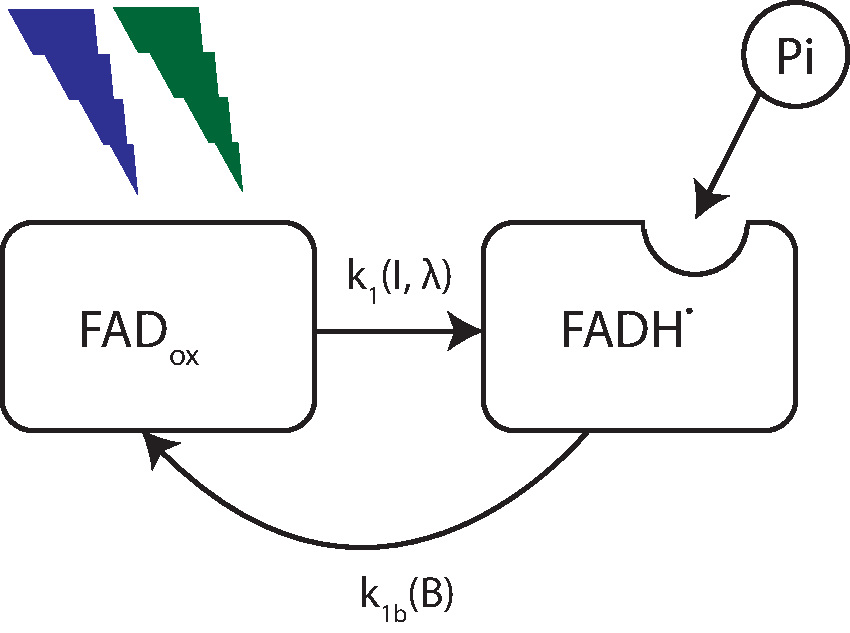
\includegraphics[width = 5cm, keepaspectratio]{photocycleTwoState.pdf}
	\caption{Photocycle for AtCRY1}
	\label{fig:photocycle}
\end{figure}

In the following it will be shown, using a combined kinetic and phosphorylation model for AtCry1, that the light-independent
re-oxidation step is magnetically sensitive. The relationship between observing a magnetic field effect, the re-oxidation rate,
light period, and dark period will be investigated for various values of light intensity where it is shown that the experimental
observations depend crucially on the above parameters chosen. That is, under certain regimes of parameters which depend strongly on
the light and dark periods, all of the magnetic protocols lead to the same result, providing no information as to which step is
magnetically sensitive.

\section{Theory}
Under the light conditions used experimentally, namely light of wavelength 450 nm, \cite{Pooam2019, Hammad2019} cryptochrome will be
reduced only to the semiquinone state $[\ce{FADH^{.}}]$ and not to the two-time reduced FADH$^-$ state, reducing the photocycle to a
two-state model \cite{Procopio2016} as illustrated in Fig.~\ref{fig:photocycle}. The time evolution of the FAD state concentrations
are then described by two simple differential equations:
\begin{subequations} \label{eq:ODE}
	\begin{align}
		\begin{split}
			\frac{d[\text{FAD}_{\text{ox}}]}{dt} & = -k_{1}(I, \lambda) [\text{FAD}_{\text{ox}}] + k_{1b}(B) [\ce{FADH^{.}}]
		\end{split}
	\\
		\frac{d[\ce{FADH^{.}}]}{dt} & = k_{1}(I, \lambda) [\text{FAD}_{\text{ox}}] - k_{1b}(B) [\ce{FADH^{.}}]
	\end{align}
\end{subequations}
Here, $k_{1}$ denotes the forward, light-dependent photoreduction rate from FADH$_{\text{ox}}$ to $[\ce{FADH^{.}}]$, and $k_{1b}$
denotes the back re-oxidation rate in the dark. In 450~nm blue light, $k_{1}$ is related to the photon fluence rate $I_{450}$ (mol
m$^{-2}$ s$^{-1}$) as follows: \cite{Kendrick94}

\begin{equation}
	k_{1} = \sigma_{450} \, I_{450} = 2.3 \, I_{450} \, \epsilon_{450} \, \Phi_{450}
\end{equation}
where $\sigma_{450}$ represents the cross section for photoconversion under 450~nm blue light, which can further be broken down into
the product of the molar extinction coefficient $\epsilon_{450}$ and quantum yield $\Phi_{450}$ at 450~nm. The photoconversion
cross-section for two-state reduction and re-oxidation of AtCry1 was determined to be $\sigma_{450} = 6.4 \times 10^{-5}$ $\mu$
mol$^{-1}$ m$^{2}$. With a fluence rate of 0.133 $\mu$ mol$^{-1}$ m$^{2} s^{-1}$ as used in the experiments,~\cite{Hammad2019} this
leads to $k_{1} = 4.8 \times 10^{-4}$ s$^{-1}$. We will use a slightly rounded rate of $k_{1} = 5 \times 10^{-4}$ s$^{-1}$ for our
calculations. The re-oxidation rate $k_{1b}$ was estimated to be around 0.01 s$^{-1}$ for the two-state photocycle of AtCry1.
\cite{Procopio2016} However, re-oxidation rates for phosphorylated AtCry1 are likely to be slower, since the addition of phosphates
will hinder the re-folding of the extended C-terminus into its closed form. We will initially assume a re-oxidation rate of $k_{1b}
= 10^{-3}$ s$^{-1}$ for our calculations and then investigate the effect of changing the re-oxidation rate.

The time dependent concentrations can be found using the algebraic constraint $[\text{FAD}_{\text{ox}}] + [\ce{FADH^{.}}] = 1$ to
reduce our system of equations in Eq.~\ref{eq:ODE} further to just one where it is assumed that one cycle of light is used. Under
these conditions, the magnetically sensitive rate, k$_{1b}$, is chosen to decrease in magnitude by 20~\%. This choice of a decrease
is motivated \cite{Hammad2019} by the fact that experimentally it is found there is an increase in the signaling state, $
[\ce{FADH^{.}}]$. This means that the concentration of $[\ce{FADH^{.}}]$ is increased, which implies k$_{1b}$ is decreased. The
strength of the magnetic field effect is justified due to the magnetic field being used, \cite{Pooam2019, Hammad2019} 500 $\mu$T.
The effect of light and magnetic fields is to alter the time in which Cry resides in the signaling state $[\ce{FADH^{.}}]$, in which
the Cry protein surface provides access to phosphorylation agents. The concurrent change in $[\ce{FADH^{.}}]$ concentration due to
the effect of a magnetic field thus contains the full quantitative information about the magnetic field effects on the photocycle
and we could, in principle, present our results in terms of the change in $[\ce{FADH^{.}}]$ concentration. However, so as to provide
an easier comparison with the experimental results, we will map these concentration differences onto a simple sigmoidal activation 
curve. This is done simply for illustrative purposes; we do not claim to have detailed information about the kinetics of 
phosphorylation. The quantitative form of the activation curve may need to be changed as more information becomes available, but
this will not affect the main conclusions from our calculations, only quantitative details.

As illustrated in Fig.~\ref{fig:photocycle}, we assume that $\ce{FADH^{.}}$ is the signalling state triggering the conformational
changes in Cry leading to phosphorylation or other further signalling steps. Because we are interested in the effects relative to
the case where there is no magnetic field (MF), we take the difference, and integrate over time to find the accumulated
concentration of our signaling state. We will refer to this as the accumulated difference, denoted by $\Delta [\ce{FADH^{.}}]$,
which is calculated as:
\begin{equation}
	\Delta [\ce{FADH^{.}}] = \int_{0}^{t_{f}} (\ce{FADH^{.}}(B) - \ce{FADH^{.}}(B = 0)) \, \mathrm{d}t.
\end{equation}

From the accumulated difference we can use the Hill equation to describe the phosphorylation binding: \cite{Phillips2009}
\begin{equation}
	p_{bound} = \frac{\left( \frac{[L]}{K_{d}} \right)^{\textsc{n}}}{1 + \left( \frac{[L]}{K_{d}} \right)^{\textsc{n}}},
	\label{eq:phosph}
\end{equation}
We choose the Hill coefficient, $N$ to be 16, which corresponds to the number of phosphorylation sites if the binding is entirely
cooperative. \cite{Phillips2009} It has been shown \cite{Liu2017} that there are as many as 24 phosphorylation sites for AtCry.
$K_{\textsc{d}}$ is a dissociation constant that sets the concentration at which half of the receptors are phosphorylated. Lastly,
[L] is the ligand concentration, which we set to correspond to the accumulated signalling state concentration difference, $\Delta
[\ce{FADH^{.}}]$. A high binding probability is indicative of an observable magnetic field effect, which we take as our ``on''
state.
As N becomes sufficiently high, the probability curve approaches a switching mechanism of on/off that allows us to identify the
presence of a magnetic field effect. That is, there will be some cutoff concentration (which is set by $K_{\textsc{d}}$, above which
the molecule will be phosphorylated, and unphosphorylated otherwise. We will later choose this value to be consistent with
experimental observation.

In all magnetic situations considered, the light is on for some time $t_{\textsc{l}}$, and then off for some time $t_{\textsc{d}}$,
which effectively switches $k_{1}$ on and off. In principle it isn't obvious which step(s) in the photocycle are magnetically
sensitive. Considerable discussion has been centered on what step in the reaction in the photocycle (see Fig~\ref{fig:photocycle})
is magnetically sensitive. Experiments have been performed that provide conclusive evidence that the back reaction, and not the
forward, is the magnetically sensitive step. As a first step, we will verify that our model captures this. Using the experimental
parameters \cite{Pooam2019} of $t_{\textsc{l}} = 300s$, $t_{\textsc{d}} = 590s$ with decay rates $k_{1b} = 10^{-3}$, $k_{1} = 4.8
\times 10^{-4}$, \cite{Procopio2016} we can calculate the phosphorylation binding using the accumulated difference for the three
scenarios described above.

Experimentally it was found that the magnetic field during the dark, and the magnetic field during the light and dark, were
indistinguishable. \cite{Pooam2019} In addition, the magnetic field effect observed with the magnetic field only on during the light
was negligible. These observations impose the following constraint:
\begin{itemize}
	\item $p_{bound}$(MF during light) < 1 \% of maximum.
	\item $p_{bound}$(MF during dark) > 90 \% of maximum
	\item $p_{bound}$(MF during light and dark) > 90 \% of maximum
\end{itemize}
These constraints can be satisfied by setting $K_{\textsc{d}} \approx 2.3$ (UNITS) leading to the sigmoidal curve shown in
Fig.\,\ref{fig:sigmoid}. Different choices of the Hill curve parameters will lead modify the quantitative details such as the
steepness of the Hill curve but does not impact the qualitative conclusions of our calculations.
\begin{figure}[h]
	\centering
	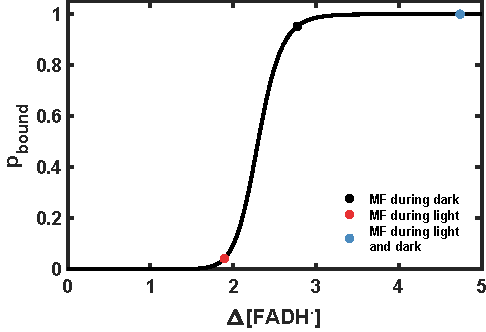
\includegraphics{sigmoid.pdf}
	\caption{Phosphorylation binding curve with $t_{\textsc{l}}$ = 300s, $t_{\textsc{d}}$ = 600s, $k_{1b} = 10^{-3}$, $k_{1} = 4.8
		\times 10^{-4}$, and phosphorylation parameters described in the text.}
	\label{fig:sigmoid}
\end{figure}

\begin{figure}[h]
	\centering
	\includegraphics[width = 8.3 cm, height = 5.553 cm]{LightMfprotocol.pdf}
	\caption{The various protocols (light on and then off for all scenarios): (a) No MF, (b) MF only during dark (c) MF only during
		light (d) MF during light and dark}
	\label{fig:protocol}
\end{figure}

\section{Results}
\begin{figure}[h]
	\centering
	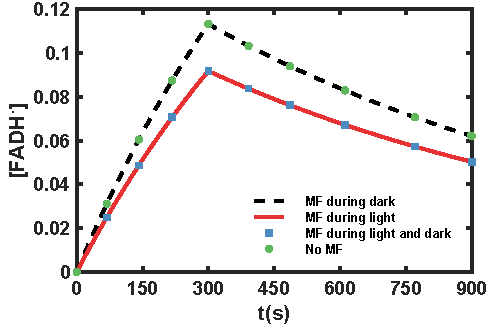
\includegraphics[width = \columnwidth, height = 5.53cm]{MfForward.pdf}
	\caption{Magnetic field effect on the forward reaction, $k_{1}$ }
	\label{fig:MfForward}
\end{figure}
With the current framework in hand, we analyze the influence of the various parameters on the magnetic field effect for the three
experimental scenarios of magnetic fields (MF during dark, MF during light, and MF during light and dark) employed in
Ref.~\cite{Pooam2019} as illustrated in Figure ~\ref{fig:protocol}

The motivation for the MF during the dark condition, as discussed above, was to provide a diagnostic test of whether the
magnetically sensitive step occurs during the forward photoreduction step, i.e., influencing k$_{1}$ in our model, or during the
re-oxidation step, i.e., influencing k$_{1b}$ in our model. If we assume that the forward rate k$_{1}$ is changed by the magnetic
field, then the experimental protocols result in the concentrations as shown in Fig.~\ref{fig:MfForward}.
\begin{figure*}[h]
	\centering
	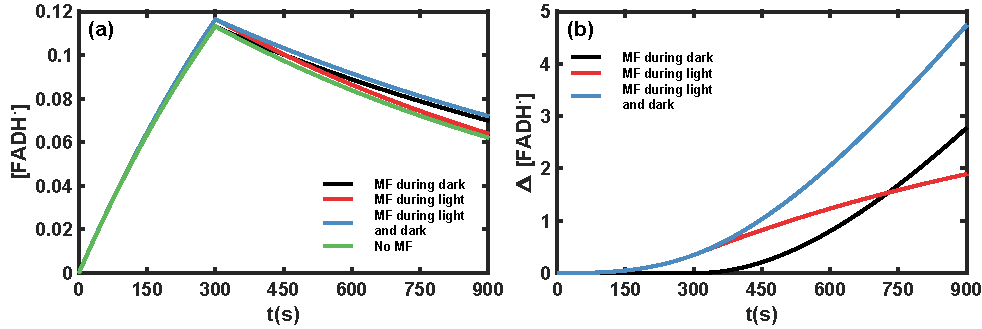
\includegraphics{concAndAccDiff.pdf}
	\caption{(a) The concentrations of the four scenarios described in the legend. (b) The accumulated differences relative to the
		no magnetic field case. In both plots $k_{1b} = 10^{-3}$, $k_{1} = 4.8 \times 10^{-4}$, and the magnetic field effect
		decreases $k_{1b}$ by 20\%.}
	\label{fig:concAndAccDiff}
\end{figure*}

In the first 300s, corresponding to $t_{\textsc{l}}$, the $[\ce{FADH^{.}}]$ concentration increases under blue light. During the
dark period $t_{\textsc{d}}$ in the remaining 600s, the concentrations reduce, but the time is not sufficient for complete
re-oxidation. As expected, applying the MF during light and dark is indistinguishable from applying the MF during light only, and
results in an increase in $[\ce{FADH^{.}}]$ concentration during the light period. Importantly, and also as expected, applying the
MF during the dark is indistinguishable from not applying a MF at all. This confirms the usefulness of applying the MF during dark
as a diagnostic tool and allows us to conclude that the experimental results on AtCry phosphorylation \cite{Pooam2019} cannot be
reconciled with the possibility of a magnetic field effect occurring \emph{only} during the forward photoreduction step.\\
\begin{figure*}[h]
	\centering
	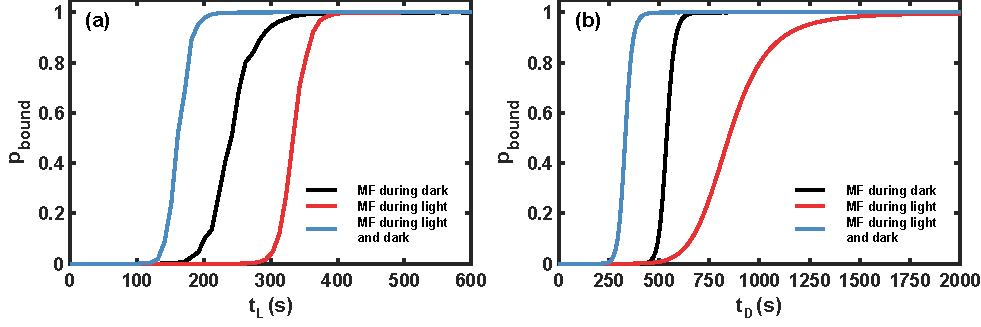
\includegraphics{varyT1T2.pdf}.
	\caption{Phosphorylation binding as a function of $t_{\textsc{l}}$ and $t_{\textsc{d}}$ with $k_{1b} = 10^{-3}$, $k_{1} = 4.8
		\times 10^{-4}$. In fig (a) $t_{\textsc{d}} = 600s$ and in fig(b) $t_{\textsc{l}} = 300s$ .}
	\label{fig:varyT1T2}
\end{figure*}

Now and in the following, we investigate MFEs on the Cry photocycle assuming that the MF changes the re-oxidation rate
$k_{1\textsc{b}}$. Fig.~\ref{fig:concAndAccDiff} shows (a) the $[\ce{FADH^{.}}]$ concentrations and, for better visibility, also (b)
the accumulated difference in $[\ce{FADH^{.}}]$ concentrations when compared to the baseline of no MF applied. During the light
period $t_{\textsc{l}}$ = 300s, an added MF enhances the $[\ce{FADH^{.}}]$ concentration because the depletion rate of this state
through re-oxidation is reduced. During the dark period, an applied MF slows down the reduction of concentration. Asymptotically,
the accumulated rate of change of $[\ce{FADH^{.}}]$ concentration is identical for the MF applied during light and dark or the MF
applied during dark only (slope of blue and black lines, respectively in Fig.~\ref{fig:concAndAccDiff}(b). However, the two curves
are offset since the effects of the MF only set in once the dark period starts, whereas they occur continuously for the MF applied
during light and dark. The effects of a MF applied are slightly more complex and, perhaps, appear counterintuitive at first sight.
Because of the MF during the light period, there is a higher concentration of $[\ce{FADH^{.}}]$ available when the light is turned
off. Even though the re-oxidation rate is no longer affected by the MF during the dark period, the $[\ce{FADH^{.}}]$ concentration
remains higher in the dark if a MF was applied during the light (red curves in Figs.~\ref{fig:concAndAccDiff}(a) and (b)) when
compared with no MF being applied. Whether or not the overall effects of the MF applied during light on the complete photocycle are
larger or smaller than the effects of the MF applied during light thus depends sensitively on the chosen parameters.

While it is easily possible to find conditions where applying the MF during light only will not yield noticeable phosphorylation
changes, whereas the other two conditions lead to saturated phosphorylation, as was observed in, \cite{Hammad2019} an increase in
the light period will eventually result in saturation of phosphorylation for the MF during light protocol as well. The choice of
experimental protocol essentially shifts the length of the light period, $t_{\textsc{l}}$, required so as to result in
phosphorylation increases. As shown in Fig.~\ref{fig:varyT1T2} (a), applying the MF during light and dark will result in the
shortest $t_{\textsc{l}}$ required for saturated phosphorylation, followed by applying the MF during dark only, with applying the MF
during light only requiring the longest period $t_{\textsc{l}}$. We note that for the light and cryptochrome parameters chosen here,
even a relatively slight increase in the light period to about 400s should be sufficient to lead to saturated phosphorylation. As
discussed above, changes in $[\ce{FADH^{.}}]$ concentration continue to accumulate in darkness even without an applied MF. This
means that an increase in dark period may also result in increased phosphorylation. For the light and Cry parameters chosen, near
saturated phosphorylation would occur for dark periods of about 1500s, about 2.5 $\times$ the length of the dark period chosen in
experimentally. \cite{Pooam2019, Hammad2019} For smaller light intensities and/or slower reoxidation rates, the initial increase in
$[\ce{FADH^{.}}]$ concentration can become insufficient to lead to phosphorylation increases for any length of $t_{\textsc{d}}$
(data not shown).
\begin{figure*}[h]
	\centering
	\includegraphics[width = 2\columnwidth]{PhosK1bTl.pdf}
	\caption{Phosphorylation binding for the three protocols, where green is the MF during the dark, purple is the MF during the
		light, and blue is the MF during dark and light (will need a better discussion/choice of color scheme). In each case, the
		light period is fixed at 300s while the dark period, and k$_{1b}$ are allowed to vary. Three cases for the rate k$_{1}$ are
		considered: (a) k$_{1} = 10^{-3}$, (b) k$_{1} = 10^{-2}$, and (c) k$_{1} = 10^{-1}$.}
	\label{fig:PvsK1bTLight}
\end{figure*}

\begin{figure*}[h]
	\centering
	\includegraphics[width = 2\columnwidth]{PhosK1bTd.pdf}
	\caption{Phosphorylation binding for the three protocols, where green is the MF during the dark, purple is the MF during the
		light, and blue is the MF during dark and light (will need a better discussion/choice of color scheme). In each case, the
		dark period is fixed at 600s while the light period, and k$_{1b}$ are allowed to vary. Three cases for the rate k$_{1}$ are
		considered: (a) k$_{1} = 10^{-3}$, (b) k$_{1} = 10^{-2}$, and (c) k$_{1} = 10^{-1}$.}
	\label{fig:PvsK1bTDark}
\end{figure*}

The parameter dependence of phosphorylation results raises the question whether there could be parameter regimes in which magnetic
field effects occur, but the protocols with MF applied only during darkness or only during light do not yield detectable changes in
$[\ce{FADH^{.}}]$ concentrations. This is particularly relevant for the usefulness of applying the MF during dark only as a
diagnostic condition. The experimenter has control over the forward photoreduction rate, $k_{1}$, through modifying the light
intensity, and over the length of light and dark periods, $t_{\textsc{l}}$ and $t_{\textsc{d}}$, but the dark re-oxidation rate,
$k_{1b}$, is a system parameter of the Cry protein in question. In the following, we will investigate the range of $k_{1b}$ for
which it is possible to achieve saturated phosphorylation in the three experimental scenarios. We will first evaluate the allowable
range of $k_{1b}$ for applying the MF during light and dark. This is essentially the reference scenario: if MF effects are found for
alternating light conditions at all, they will occur in this scenario. We indeed find that in all cases studied, the parameter range
for which phosphorylation can be achieved for the MF during dark and light scenario encompasses the parameter ranges for which
saturation phosphorylation can be achieved in the other two scenarios.

We first set the light period $t_{\textsc{l}}$ to 300 s, as employed in the experiments, and vary both the unknown reoxidation rate,
the dark period $t_{\textsc{d}}$ and the forward photoreduction rate $k_{1}$, the latter being essentially a measure for the light
intensity employed in the experiment. Fig.~\ref{fig:PvsK1bTLight} shows the parameter ranges for which saturation phosphorylation
can be achieved in the three scenarios. We note an upper and lower bound for the dark reoxidation rate $k_{1b}$ so as to achieve
saturation phosphorylation. If $k_{1b}$ is low, one needs to wait increasingly longer times for MFE to accumulate. On the other
hand, if $k_{1b}$ is high, the signaling state will be depleted quickly, also reducing the MFE effects. The upper bound depends
strongly on the relationship of the forward photoreduction rate $k_{1}$ and the reoxidation rate $k_{1b}$. Once the reoxidation rate
$k_{1b}$ is more than about 10 times faster than the photoreduction rate $k_{1}$, the MFEs on phosphorylation disappear. 

We will then compare the allowable range of $k_{1b}$ for applying the MF during dark only, or MF during light only.

\emph{leaving old stuff here for now}
If instead we allow $t_{\textsc{l}}$ and $k_{1b}$ to vary, as in Fig.\,\ref{fig:PvsK1bTLight}, we find various regions that
experimental observations can use to narrow $k_{1b}$ within some range.

Lastly, if we consider the case of allowing $t_{\textsc{d}}$ and $k_{1b}$ to vary, as in Fig.\,\ref{fig:PvsK1bTDark}, we again see
various regions emerge. In both situations, it appears that the MF during only the dark places the largest restriction on the
available range of $k_{1b}$. There also exists a value of $k_{1b}$ above which no phosphorylation can occur, and depends on how the
magnetic field is applied.

\section{Discussion}
First kinetic model study on alternating light/dark effects.

Alternating light/dark protocol is useful. Applicable in virtually the same range that MFE occur.

Does not rule out MF on forward photoreduction. Did not study combined effects here.

Applying MF during light only is less applicable, depends strongly on parameters. \cite{Hammad2019} may have been fortunate in
choice of conditions.

Need to model effects of repeated cycling, especially for bird results.
Although the precise model for phosphorylation binding for AtCRY1, and the photocycle parameters, are unknown, the qualitative
features shown above are generally applicable. Our conclusions are valid over a fairly wide range of models incorporating
cooperativity, as long as there is a sufficiently sharp transition between phosphorylated and unphosphorylated. In principle, it
isn't immediately obvious why the scenario with the magnetic field on
Discuss how the plots could be used to narrow down the range of k1b by looking at orientation for various time/MF pulses
It's possible that the experimental set of parameters chosen, light intensity, light and dark periods, were responsible for the
observations of the MF during the dark, and MF during the light and dark, produce the same results, while the MF during only the
light produced a negligible response.
Complicated interplay between the light/dark periods with back reaction rate.
Discuss that the kinetic + binding model are consistent with the experimental conclusion that the magnetically induced step is in
the back-reaction
Discuss connection of number of phosphorlyation sites with how much we can constrain ?

\section{Conclusions}
A simple model has been proposed to  understand the experimental observation that there is no distinguishable difference between
applying the magnetic field only during the dark versus during the light and dark periods. In addition, the relationship between
phosphorylation binding and light/dark periods was investigated and found that the scenario of MF on only during the dark may
provide a diagnostic test for determining $k_{1b}$.

\section*{Conflicts of interest}
There are no conflicts to declare.

\section*{Acknowledgements}
The Acknowledgements come at the end of an article after Conflicts of interest and before the Notes and references.

%%%END OF MAIN TEXT%%%

%The \balance command can be used to balance the columns on the final page if desired. It should be placed anywhere within the
first column of the last page.

\balance

%If notes are included in your references you can change the title from 'References' to 'Notes and references' using the following
command:
%\renewcommand\refname{Notes and references}

%%%REFERENCES%%%
\bibliographystyle{unsrt} %the RSC's .bst file
\bibliography{C:/Users/shawn/Desktop/references}



\end{document}
